\documentclass[11pt]{article}
\usepackage{amsmath}
\usepackage{graphicx}
\usepackage{hyperref}
\usepackage[utf8]{inputenc}
\usepackage[spanish]{babel}
\usepackage[margin=2cm]{geometry}
\usepackage{amsfonts}
\usepackage{listings}
\usepackage[T1]{fontenc}
\usepackage{float}
\usepackage{subfig}

\title{Práctica 2 Minería de Texto - Minería de Medios Sociales.}
\author{Curso: 2018/2019. Néstor Rodríguez Vico. DNI: 75573052C - \href{mailto:nrv23@correo.ugr.es}{nrv23@correo.ugr.es}}
\date{\today}

\lstdefinestyle{bash_style}{
	language=bash,
	frame=single,
	xleftmargin=.25in,
	upquote = true,
	basicstyle=\scriptsize,
	breakatwhitespace=false,         
	breaklines=true,                 
	captionpos=b,                    
	keepspaces=true,                 
	numbers=left,                    
	numbersep=5pt,                  
	showspaces=false,                
	showstringspaces=false,
	showtabs=false,                  
	tabsize=2
}

\lstset{style=bash_style}

\begin{document}
\maketitle

\section{Clasificación.}

Primero he resuelto la parte de clasificación. Para ello, he cogido el \textit{workflow} \textit{Sentiment Classification} proporcionado por el profesor de la asignatura y lo he modificado para añadir dos nuevos clasificadores. El \textit{workflow} resultante es el siguiente:

\begin{figure}[H]
	\centering
	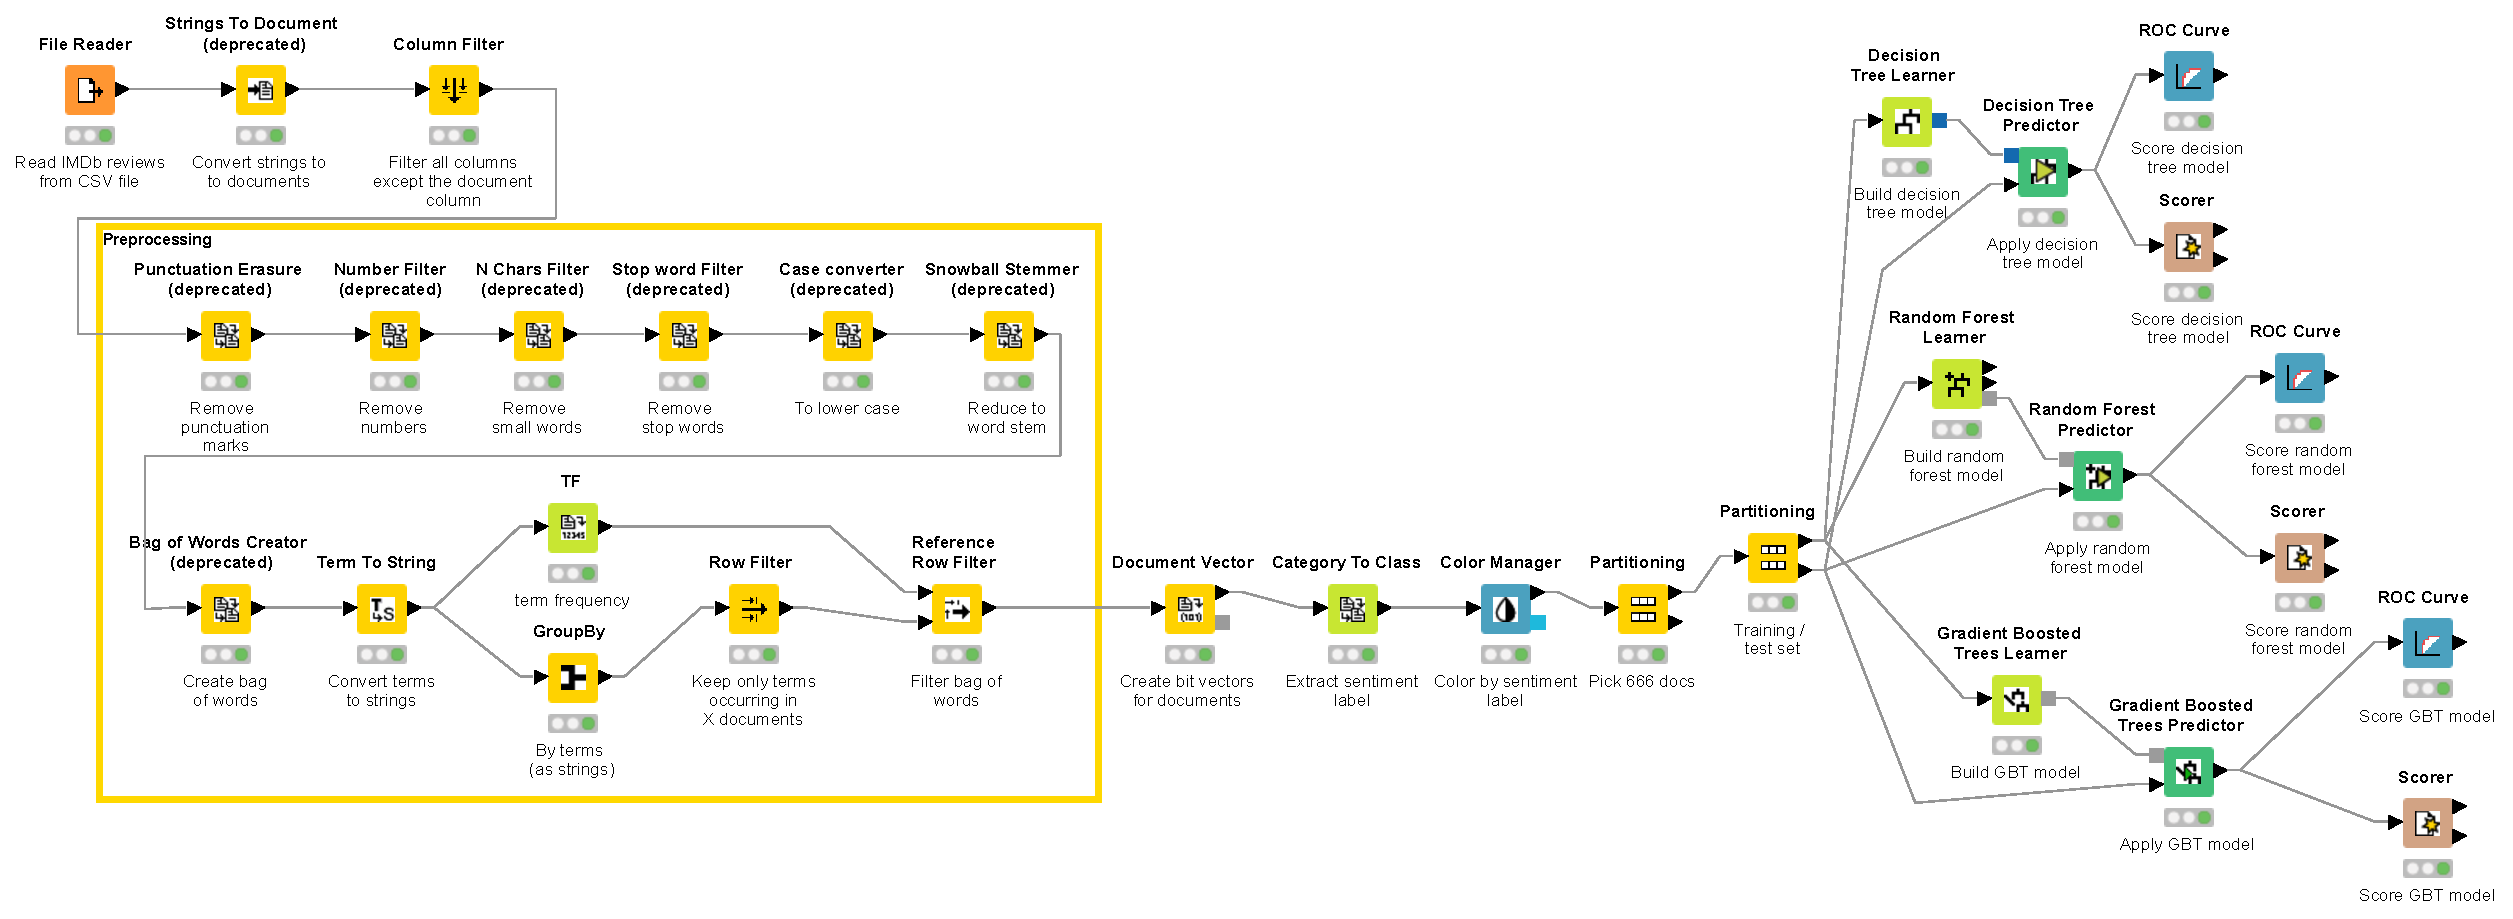
\includegraphics[width=\linewidth]{images/class_wf.eps}
\end{figure}

Se han añadido los siguientes nodos:

\begin{itemize}
	\item \textit{Random Forest Learner}: Dicho nodo implementa un algoritmo \textit{Random Forest}.
	\item \textit{Random Forest Predictor}: Una ves hemos aprendido un modelo \textit{Random Forest}, usamos este nodo para realizar la predicción.
	\item \textit{Scorer (1)}: Evaluamos como ha ido la predicción del modelo \textit{Random Forest}.
	\item \textit{Gradient Boosted Trees Learner}: Dicho nodo implementa un algoritmo \textit{Gradient Boosted Trees}.
	\item \textit{Gradient Boosted Trees Predictor}: Una ves hemos aprendido un modelo \textit{Gradient Boosted Trees}, usamos este nodo para realizar la predicción.
	\item \textit{Scorer (2)}: Evaluamos como ha ido la predicción del modelo \textit{Gradient Boosted Treest}.
\end{itemize}

El preprocesamiento seguido es el mismo que había en el \textit{workflow} proporcionado por el profesor. Los pasos son:

\begin{itemize}
	\item Eliminar signos de puntuación.
	\item Eliminar números.
	\item Eliminar palabras pequeñas.
	\item Eliminar \textit{stopwords}.
	\item Convertir a minúsculas.
	\item Quedarnos con la raiz de las palabras.
	\item Construimos la bolsa de palabar y convertimos los términos a \textit{strings}.
	\item Calculamos la frecuencia de términos (\textit{tf}) y nos quedamos sólo con los términos que aparecen en, al menos, 20 documentos.
	\item Finalmente, filtramos la bolsa de palabras.
\end{itemize}

Como podemos ver en medio del \textit{workflow}, hay dos nodos \textit{partitioning}. El segundo de ellos es para separar el conjunto de datos en un conjunto de \textit{train} (\textit{70\%} de las instancias) y \textit{test} (\textit{30\%} de las intancias). El primero de ellos lo que hace ese seleciconar \textit{666} documentos de forma estratíficada. Esto se ha hecho para tener \textit{200} instancias en el conjunto de \textit{test}, ya que es el número máximo de instancias que he podido ejecutar en la segunda parte de la práctica (comentaré los detalles en dicha sección). Los resultados obtenidos son los siguientes: 

\begin{table}[H]
	\centering
	\begin{tabular}{rcc}
		\textbf{Modelo} & \textbf{\% Acierto} & \textbf{Kappa} \\ \hline
		\textbf{Decision Tree} & 83.5 & 0.67 \\
		\textbf{Random Forest} & 85.0 & 0.70 \\
		\textbf{Gradient Boosted Trees} & 89.0 & 0.78
	\end{tabular}
\end{table}

Como podemos ver, el mejor resultado lo obtenemos con el algoritmo \textit{Gradient Boosted Trees}.

\section{Análisis de sentimientos.}

Para resolver esta parte he cogido el \textit{workflow} \textit{Sentiment Analysis} proporcionado por el profesor de la asignatura y lo he modificado adaptarlo al enunciado. El \textit{workflow} resultante es el siguiente:

\begin{figure}[H]
	\centering
	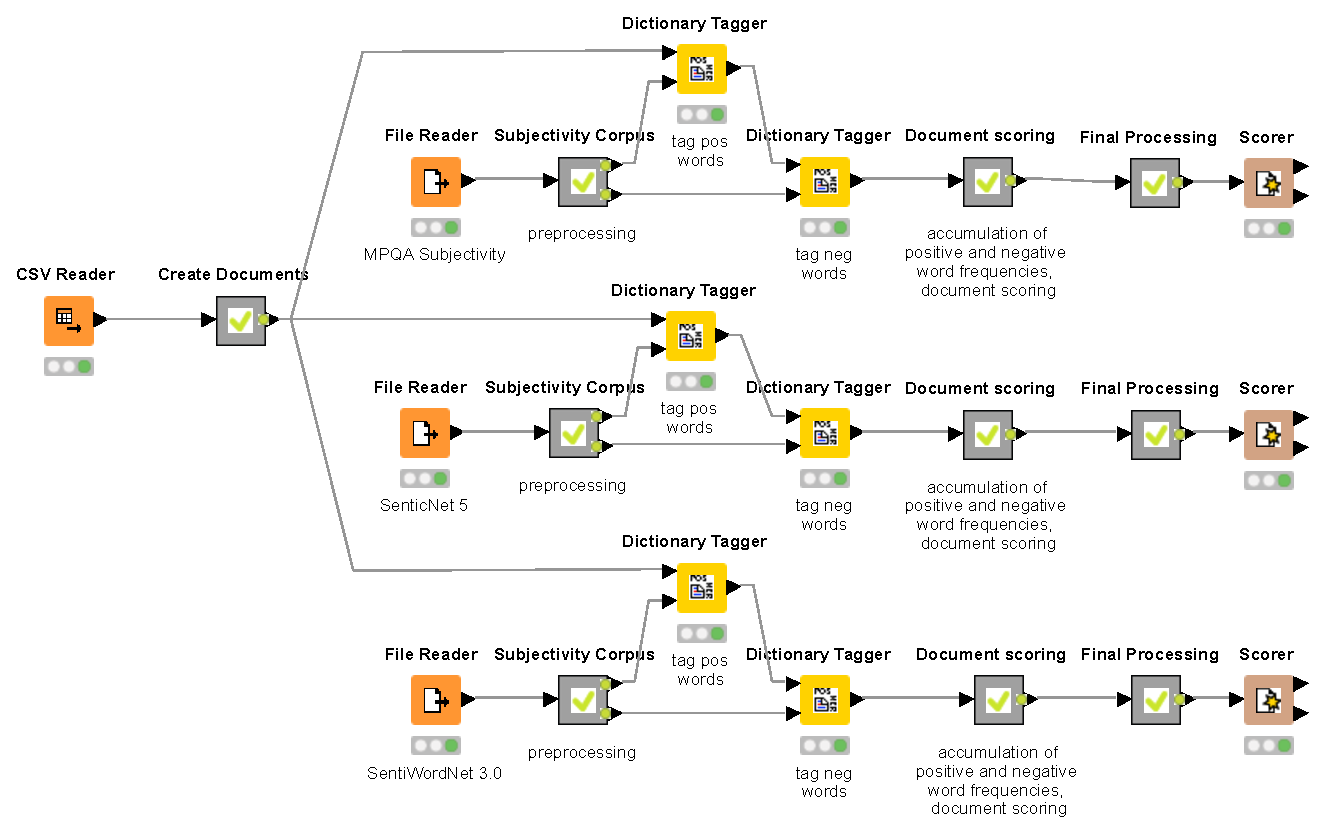
\includegraphics[width=\linewidth]{images/analysis_wf.eps}
\end{figure}

Las diferentes partes del \textit{workflow} son:

\begin{itemize}
	\item En la primera parte podemos ver la parte común a las tres ramas posteriores. Dicha parte se encarga de leer el conjunto de datos, y ejecutar el nodo \textit{Create Documents}. Dicho nodo es el siguiente:
	
	\begin{figure}[H]
		\centering
		\includegraphics[width=0.5\linewidth]{images/create_documents.png}
	\end{figure}
	
	Dicho nodo agrupa por identificador (por si hay varios documentos con el mismo identificador) y convierte el texto leido a una variable de tipo \textit{Document}, que es la usada por \textit{KNIME} para representar un documento. A continuación, cogemos los mismos \textit{666} documentos que hemos cogido en la práctica de Clasificación y dividimos el conjunto de dichos documentos en train y test. Tanto en la parte de clasificación como en la parte de análisis de sentimientos se han usado las mismas semillas, lo cual nos garantiza que el conjunto de documentos usado como conjunto de test en la parte de clasificación es el mismo conjunto de instancias que estamos usando en la parte de análisis, pudiendo hacer así una comparación justa. Como comenté anteriormente, para este \textit{workflow} he usado \textit{200} documentos sólo. Esto se debe a que, por problemas de rendimiento de mi máquina, no he podido ejecutar el \textit{workflow} para más elementos.
	
	\begin{itemize}
		\item La primera rama hace uso del \textit{lexicon} \textit{MPQA Subjectivity}. Tras leer el \textit{lexicon}, he aplicado preprocesamiento. Dicho preprocesamiento es el siguiente:
		
		\begin{figure}[H]
			\centering
			\includegraphics[width=0.8\linewidth]{images/MPQA_preprocessing.png}
		\end{figure}
		
		Este preprocesamiento consiste en utilizar nodos del tipo \textit{Java Snippet} para parsear las columnas del \textit{corpus} eliminando los símbolos \textit{igual} (\textit{=}) de cada columna para quedarnos sólo con la información relevante. A continuación, separamos el conjunto de documentos en documentos con sentimiento positivo (salida superior del nodo) y documentos con sentimiento negativo (salida inferior del nodo).
		\item La segunda rama hace uso del \textit{lexicon} \textit{SenticNet 5}. Tras leer el \textit{lexicon},, he aplicado preprocesamiento. Dicho preprocesamiento consiste en separar el conjunto de documentos en documentos con sentimiento positivo (salida superior del nodo) y documentos con sentimiento negativo (salida inferior del nodo).
		\item La tercera rama hace uso del \textit{lexicon} \textit{SentiWordNet 3.0}. Para poder leer correctamente dicho \textit{lexicon}, he hecho un script en \textit{Python} \footnote{Dicho \textit{script} no se ha entregado. Si lo desea, hágamelo saber y se lo mando.} para formatear un poco el \textit{lexicon}. El problema que tienes dicho lexicon es en la columna \textit{SynsetTerms}. Dicha columna contiene el término en cuestión, el problema es que puede contener una lista de términos, los cuales son sinónimos entre ellos. Por lo tanto, lo que he hecho es repetir cada fila tantas veces como términos haya dejando en cada fila un único término. Tras leer el \textit{lexicon}, he aplicado preprocesamiento. Dicho preprocesamiento es el siguiente:
		
		\begin{figure}[H]
			\centering
			\includegraphics[width=0.5\linewidth]{images/SentiWordNet_preprocessing.png}
		\end{figure}
		
		Lo primero que hacemos es usar un nodo \textit{Java Snippet}. Dicho nodo lo que hace es calcular la polaridad de las palabras del \textit{lexicon}, ya que este no nos las da, sino que nos da una intensidad de positividad y otra de negatividad. Lo que he hecho es considerar una polaridad positiva si la intensidad de positividad es mayor que la intensidad de negatividad y una polaridad negativa en caso contrario. A continuación, separo el conjunto de documentos en documentos con sentimiento positivo (salida superior del nodo) y documentos con sentimiento negativo (salida inferior del nodo).
	\end{itemize}

	\item Una vez tenemos la estructura del \textit{corpus} lista, realizamos los mismos pasos para todos ellos. Los dos primeros nodos son nodos de etiquetado (\textit{Dictionary Tagger}), los cuales sirven para etiquetar las elementos de los documentos en base al \textit{corpus} usado.
	\item El siguiente paso es puntuar el documento. Para ello hacemos uso del \textit{metanodo} \textit{Document Scoring}. Dicho nodo es similar al presente en el \textit{workflow} original. En dicho nodo hacemos lo siguiente:
	
	\begin{figure}[H]
		\centering
		\includegraphics[width=0.9\linewidth]{images/document_scoring.png}
	\end{figure}
	
	Primero se construye una bolsa de palabras y filtrmos los términos no deseados, calculamos la frecuencia de términos (\textit{tf}), convertimos las etiquetas a \textit{strings}, agrupamos la salida por términos e imputamos los valores de frecuencia de términos perdidos si los hubiese. Finalmente, renombramos las columnas para que sea más fácil hacer referencias a ellas posteriormente.
	
	\item A continuación, llamamos al metanodo \textit{Final Processing}. Dicho nodo hace lo siguiente:
	
	\begin{figure}[H]
		\centering
		\includegraphics[width=0.9\linewidth]{images/final_processing.png}
	\end{figure}
	
	En el nodo \textit{GroupBy} agrupamos por documentos. En el nodo \textit{Java Snippet} sumamos la puntuación de los término dentro de cada documentos y ordenamos el resultado con el nodo \textit{Sorter}. En el siguiente nodo \textit{Java Snippet} lo que hacemos es cambiar el valor numérico de la puntuación por una etiqueta. Si dicha puntuación es mayor que cero la etiqueta será \textit{POS}, \textit{NEG} en caso contrario. El segundo nodo \textit{Java Snippet} convierte la variable que almacena el documento a una variable de tipo \textit{String}, para poder manipularla correctamente en etapas futuras. Finalmente, agrupamos por documento para obtener la etiqeuta predicha de cada uno de los documentos y  renombramos las columnas para que sea más fácil identificar que representa cada una de ellas.
	
	\item Una vez tenemos la etiqueta predicha y la etiqueta real, usamos el nodo \textit{Scorer} para compararlas y sacar las métricas que se muestran a continuación.
\end{itemize}

Los resultados obtenidos son los siguientes: 

\begin{table}[H]
	\centering
	\begin{tabular}{rcc}
		\textbf{Lexicon} & \textbf{\% Acierto} & \textbf{Kappa} \\ \hline
		\textbf{MPQA Subjectivity} & 70.5 & 0.399 \\
		\textbf{SenticNet 5} & 53.0 & 0.011 \\
		\textbf{SentiWordNet 3.0} & 62.7 & 0.018
	\end{tabular}
\end{table}

Como podemos ver, los mejores resultados los obtenemos con el lexicon \textit{MPQA Subjectivity}, el cual obtiene unos resultados bastante mejores que los obtenidos con los otros dos lexicones.

\section{Comparación.}

Tal y como he comentado en la sección de análisis, cuando se han seleccionado los documentos, se ha garantizado que el conjunto de \textit{test} en la parte de clasificación contiene los mismos documentos que el conjunto usado en la parte de análisis. A continuación podemos ver una tabla comparativa de los resultados obtenidos aplicando las distintas técnicas

\begin{table}[H]
	\centering
	\begin{tabular}{rcc}
		\textbf{Modelo} & \textbf{\% Acierto} & \textbf{Kappa} \\ \hline
		\textbf{Decision Tree} & 83.5 & 0.67 \\
		\textbf{Random Forest} & 85.0 & 0.70 \\
		\textbf{Gradient Boosted Trees} & 89.0 & 0.78 \\ \hline
		\textbf{Media} & 85.866 & 0.716 \\
		\textbf{} &  &  \\
		\textbf{Lexicon} & \textbf{\% Acierto} & \textbf{Kappa} \\ \hline
		\textbf{MPQA Subjectivity} & 70.5 & 0.399 \\
		\textbf{SenticNet 5} & 53.0 & 0.011 \\
		\textbf{SentiWordNet 3.0} & 62.7 & 0.018 \\ \hline
		\textbf{Media} & 62.066 & 0.142
	\end{tabular}
\end{table}

Cómo podemos ver, las técnicas de clasificación son bastante mejores, obteniendo un porcentaje de acierto del \textit{85.866\%} en media frente al \textit{62.066\%} en media obtenido por las técnicas de análisis.

\end{document}